\section{Propuesta}
\label{sec:propuesta}

La propuesta consiste en desarrollar una red dinamica eficiente que
sea robusta ante posibles fallas en la interconexión física de los
datacenters. Para esto se ha desarrollado un modelo basado
probabilístico que asegura el total funcionamiento de la red para un
cierto umbral de seguridad.

\begin{figure}[h]
\centering
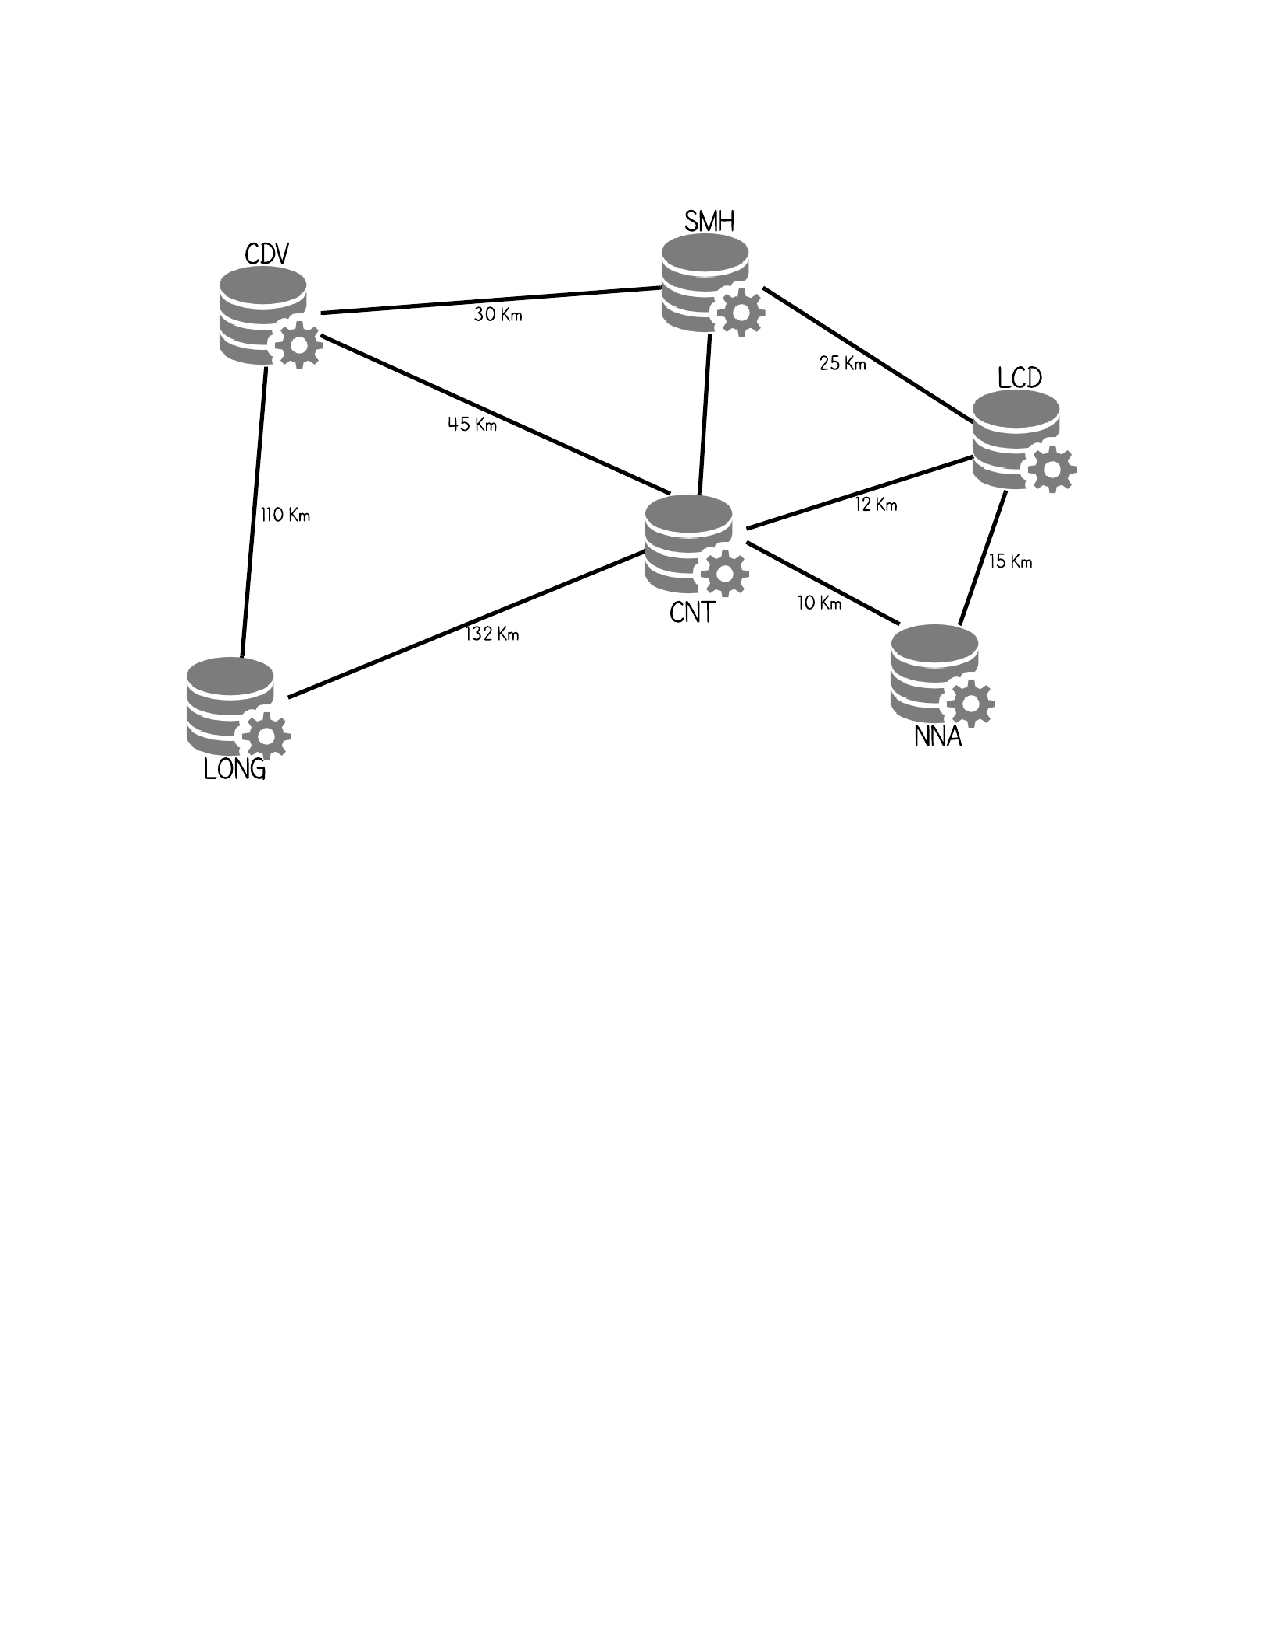
\includegraphics[width=0.7\textwidth]{Imagenes/datacenters.pdf}
\caption{Diagrama d}
\end{figure}

Para la definición de la red, fue necesario definir las rutas que
conectan cada par de \textit{DataCenters}.  Para obtener un modelo
robusto a cortes, es necesario que exista más de una ruta entre cada
par de puntos o almenos cierta cantidad que garantize los
requerimientos predefinidos.

La forma en que se diseño esta red, utiliza ciertas características
intrínsicas de la red de fibra oscura actual. Por ejemplo se ciñe a
las tasas anuales de corte para la fibra utilizada (AEG-10
\textbf{CORREGIR}), y también a las capacidades requeridas por cada
protocolo GE y (balblalbal)


El conjunto de rutas alternativas debe cumplir un criterio de umbral
de seguridad, si no lo cumple se agregarán más rutas alternativas
hasta que se logre dicho objetivo.
